

\begin{figure}[!h]
    \centering
    \resizebox{0.86\textwidth}{!}{
        \begin{tikzpicture}[mindmap,
        level 1 concept/.append style={level distance=130,sibling angle=120},
        level 2 concept/.append style={level distance=80,sibling angle=120},
        level 3 concept/.append style={level distance=70,sibling angle=120},
        level 3 concept/.append style={level distance=60,sibling angle=120},
        ]
        \path[mindmap,concept color=black,text=white]
        node[concept] {Angles}
        [clockwise from=0]
        child[concept color=green!50!black,sibling angle=180,text=black] {
            node[concept] (angleMeasurement) {Measurement}
            [clockwise from=90]
            child[concept color=green!50!black,sibling angle=180] {
              node[concept] (radians) {Radians}
            }
            child[concept color=green!50!black,sibling angle=180] {
              node[concept] (degrees) {Degrees}
            }
        }
        child[concept color=blue,sibling angle=120,text=black]{
          node[concept] (unitCircle) {Arcs}
          [clockwise from=0]
          child[concept color=blue] {
            node[concept] (arcLength) {Arc Length}
          }
          child[concept color=blue,sibling angle=65] {
            node[concept] (arcArea) {Arc Area}
          }
        }
        child[concept color=red,sibling angle=120,text=black]{
          node[concept] (unitCircle) {Unit Circle}
          [clockwise from=90]
          child[concept color=red] {
            node[concept] (trigFunctions) {Trigonometric Functions}
            [counterclockwise from=0]
            %child { node[concept] (rangeDomain) {Range / Domain} }
            child[sibling angle=90] {
              node[concept] (sine) {Sine}
              [counterclockwise from=-22]
              child[sibling angle=45] {node[concept] {Range}}
              child[sibling angle=45] {node[concept] {Domain}}
              }
            child[sibling angle=90] {
              node[concept] (cosine) {Cosine}
              [counterclockwise from=68]
              child[sibling angle=45] {node[concept] {Range}}
              child[sibling angle=45] {node[concept] {Domain}}
              }
            child[sibling angle=90] {
            node[concept] (tangnet) {Tangent}
            [counterclockwise from=158]
            child[sibling angle=45] {node[concept] {Range}}
            child[sibling angle=45] {node[concept] {Domain}}
            }
          }
        };

        \begin{pgfonlayer}{background}
        \draw [left color=red, right color=green, draw=white,
               decorate,decoration=circle connection bar]
               (trigFunctions) -- (radians);
        %\draw [left color=blue, right color=green!50!black, draw=white,
        %       decorate,decoration=circle connection bar]
        %       (arcLength.east) -- (radians.east);
        \draw [color=blue,ultra thick,looseness=1.5,<->] (arcLength) [out=-22, in=-45] to (radians);
        %\draw [left color=blue, right color=green!50!black, draw=white,
        %       decorate,decoration=circle connection bar]
        %       (arcArea.east) -- (radians.east);
        \draw [color=blue,ultra thick,looseness=1.5,<-] (arcArea) [out=0, in=-45] to (radians);
        \end{pgfonlayer}


        \end{tikzpicture}
    }
\caption{Topics for the section on angles.}
  \end{figure}



\preClass{Coordinate Systems}

\videoLink{Section 4.1}{https://www.youtube.com/playlist?list=PLYHZK3b8UFw3HtpDsf1SA0Znm5\_7bAGBY}

\begin{enumerate}
\item  Convert the following angles measured in degrees to radian measure.  Your answers must be written as fractions and not rounded decimals.
\begin{enumerate}
\item $\theta=60^\circ$\vfill
\item $\beta=110^\circ$\vfill

\end{enumerate}

\item  Find one positive angle and one negative angle that is coterminal to $\displaystyle \theta=\frac{3}{2}\pi$.\vfill

\newpage

\item Answer the following questions about a circle that has radius 7 and an angle $\theta$ that subtends an arc of length 15.
\begin{enumerate}
\item Determine $\theta$ in radians and degrees.\vfill
\item Determine the area of the circular sector with central angle $\theta$ found in part $(a)$.\vfill
\end{enumerate}


\end{enumerate}






\actTitle{Worksheet 4.1}


\noindent \textbf{Instructions:}  Work together in groups of  3 or 4 to complete the following problems.\\

Student goals:
\begin{itemize}
\item Determine an angle's measurement in radians given the arc length
  and radius of a sector.
\item Place an angle in standard position given a verbal description.
\item Determine the terminal or the initial side of a sector.
\item Recognize whether an angle is positive, negative or zero.
\item Recognize when two angles have coterminal sides.
\item Given any two values of a sector's radius, angle, or arc length
  determine the value of the remaining quantity.
\item Determine the area of a sector given the radius and angle.
\item Given any two values of a sector's radius, angle, or arc length
  determine the value of the area of the sector.
\item Recognize when a given angle represents more than one complete
  rotation around a circle.
\end{itemize}


For each of the following questions first make a rough sketch of the
relevant figure.
\begin{enumerate}

\item Find a positive angle less than $360^\circ$ that is coterminal with each of the given angles.
\begin{enumerate}
\item  $\theta=400^\circ$\vfill
\item $\alpha=-160^\circ$\vfill
\vfill
\end{enumerate}


\item Find a positive angle less than $2\pi$ that is coterminal with each of the given angles.
\begin{enumerate}
\item  $\displaystyle \beta=-\frac{\pi}{15}$\vfill
\item $\displaystyle \phi=\frac{34\pi}{9}$\vfill
\vfill
\end{enumerate}

\clearpage

\item Find the radian measure of the central angle $\theta$ of a circle of radius $r=8$ meters that intercepts an arc of length $s=14$ meters.
\vfill


\item The minute hand of a clock is 3 inches long.  How far does the tip of the minute hand move in 45 minutes?\vfill

  \clearpage
  
\item The minute hand of a clock moves from 12:10 to 12:30.
\begin{enumerate}
\item How many \textbf{degrees} does it move during this time?\vfill
\item How many \textbf{radians} does it move during this time?\vfill
\item If the minute hand is 10 inches in length, determine the exact distance the tip of the minute hand travels during this time.\vfill
\end{enumerate}

\item Find the exact area of the following sectors given the radius of
  the circle $r$ and the subtended angle $\theta$.  Then round the
  result to the nearest tenth of a unit.

\begin{enumerate}
\item $r=6$ m; $\theta=\frac{5\pi}{3}$\vfill
\item $r=3$ cm; $\theta=120^\circ $\vfill

\end{enumerate}


\clearpage

\item You are one member of a group of 8 friends who are going out for pizza.  A small pizza has a 6" radius, while a large pizza has 9"  radius.  Answer the following questions.
\begin{enumerate}
	\item How much pizza will each of you eat if you order two small pizzas?  Will you get more of less pizza if you order one large pizza? (Assume everyone eats the same amount and all the pizza is eaten.)
	\vfill
	\item How many inches of crust will each person eat if you order two smalls?  If you order one large will you get more crust?
	\vfill
	\item Suppose you and your friends want to order one pizza and that you each want to eat 50 square inches worth of pizza.  What should the radius of the pizza be?
	\vfill
\end{enumerate}

\clearpage

\item The radius of the circle shown in the diagram below is three, and
  the area of the sector defined by the shaded region is 10.5.
  Determine the radian measure of the angle $\psi$.

  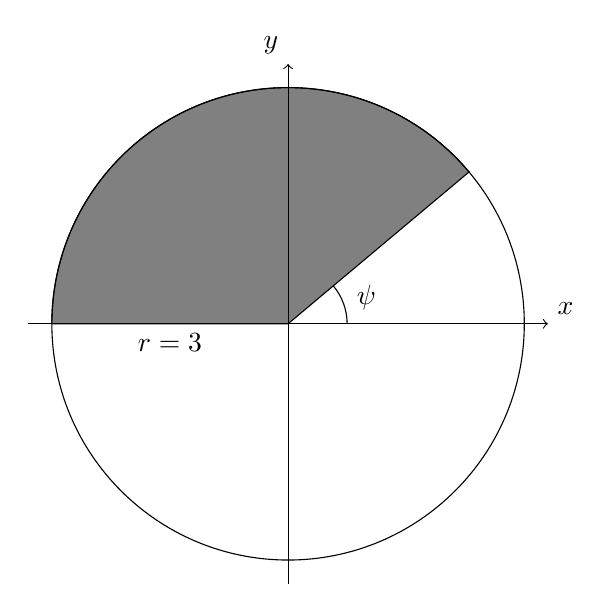
\begin{tikzpicture}[y=1.5cm, x=1.5cm,font=\sffamily]
    \draw[thin,black,fill=gray] (0,0) -- (40:2) arc (40:180:2) -- (0,0);
    %\draw[very thick,black] (40:2) arc (40:180:2);
    \draw[black] (0,0) circle (2);
    \draw[black] (0:.5) arc (0:40:.5) node[pos=0.1,anchor=south west] {$\psi$};
    % \node[xshift=0] at (145:0.7) {$\delta$};
    % \draw[thin,black] (110:0.3) arc (110:180:0.3);
    \draw[thin,black,->] (-2.2,0.0) -- (2.2,0.0) node[anchor=south west] {$x$};
    \draw[thin,black,->] (0.0,-2.2) -- (0.0,2.2) node[anchor=south east] {$y$};
    \node[black,anchor=north] at (-1,0) {$r=3$};
    % \node[black,anchor=south west] at (55:2) {$s$};
  \end{tikzpicture}

  \vfill

\item A wheel with a diameter of 0.7m rolls a distance of 400m. What angle did it turn?

  \vfill
    

\end{enumerate}


\hwTitle{Section 4.1}

\begin{enumerate}
\item Suppose that the three circles drawn below have radii of length
  1, 2, and 3. You can move from one point to the other only by moving
  along the segments shown in the diagram.  For each pair of points
  given below, find the shortest path connecting the points.
%\vspace{-1in}
\begin{center}
  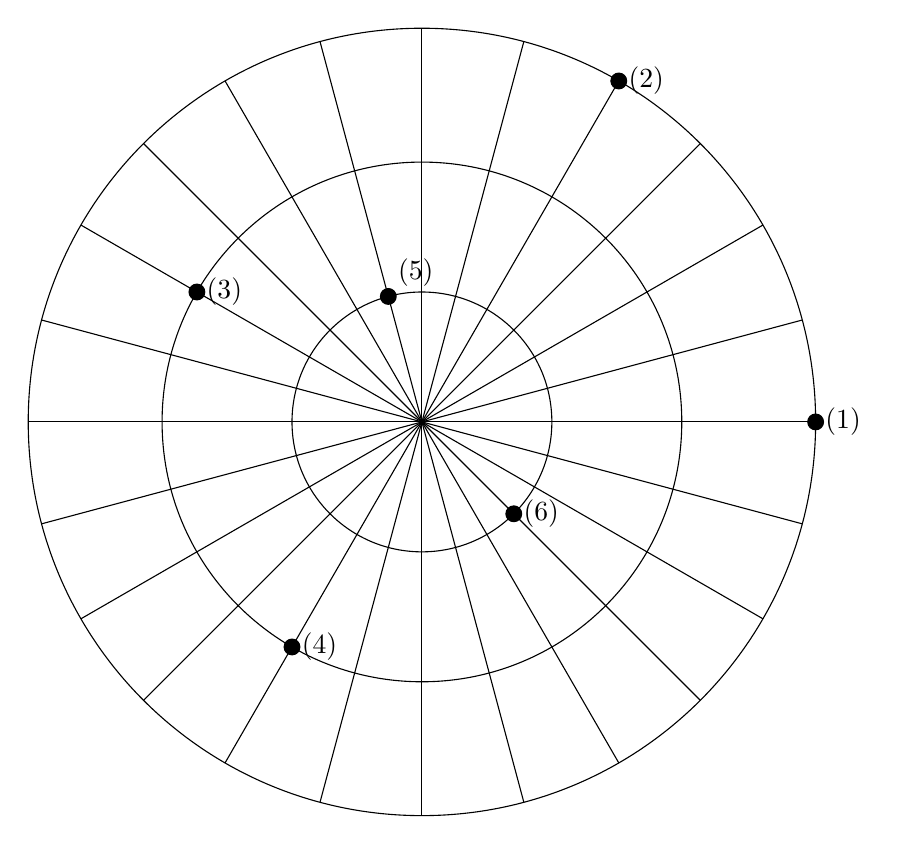
\begin{tikzpicture}[scale=5]
    \foreach \t in {0,15,30,...,345} {
      \draw[-] (0,0) -- (\t:1);
    }   
    \draw (0,0) circle(1);
    \draw (0,0) circle(0.66);
    \draw (0,0) circle(0.33);
    \filldraw[black] (1,0) circle (0.02) node[anchor=west] {(1)};
    \filldraw[black] (60:1) circle (0.02) node[anchor=west] {(2)};
    \filldraw[black] (150:0.66) circle (0.02) node[anchor=west] {(3)};
    \filldraw[black] (240:0.66) circle (0.02) node[anchor=west] {(4)};
    \filldraw[black] (105:0.33) circle (0.02) node[anchor=south west] {(5)};
    \filldraw[black] (315:0.33) circle (0.02) node[anchor=west] {(6)};
  \end{tikzpicture}
\end{center}



%\vspace{-1in}
\begin{enumerate}
\begin{multicols}{3}
	\item From (1) to (2).
	\item From (3) to (4).
	\item From (5) to (6).
	\item From (3) to (5).
	\item From (2) to (4), \\
	avoiding the center
\end{multicols}
\end{enumerate}




\item Find the exact area of the following sectors given the radius of
  the circle $r$ and the subtended angle $\theta$.  Then round the
  result to the nearest tenth of a unit.
  \begin{enumerate}
  \item $r=1.2$ ft; $\theta=\frac{\pi}{6}$
  \item $r=2.1$ ft; $\theta=\frac{11\pi}{6}$
  \end{enumerate}

\item Determine the function that returns the angle of a sector of
  radius 5 given the area of the sector. If you double the area what
  happens to the angle?
\item Determine the function that returns the angle of a sector of
  radius 8 given the arclength of the sector. If you double the
  arclength what happens to the angle?

\item The radian measure of the angle $\psi$ is $\frac{\pi}{4}$, and
  the area of the sector defined by the shaded region is 11.
  Determine the radius of the circle. If the area is increased how
  does the radius change? \\ 
  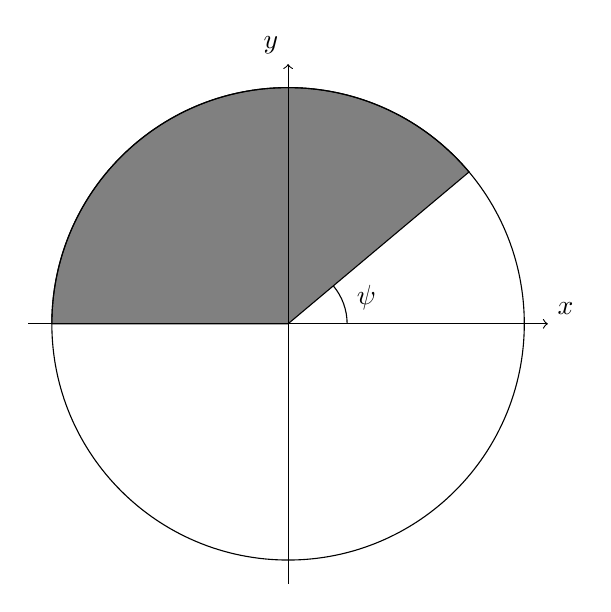
\begin{tikzpicture}[y=1.5cm, x=1.5cm,font=\sffamily]
    \draw[thin,black,fill=gray] (0,0) -- (40:2) arc (40:180:2) -- (0,0);
    %\draw[very thick,black] (40:2) arc (40:180:2);
    \draw[black] (0,0) circle (2);
    \draw[black] (0:.5) arc (0:40:.5) node[pos=0.1,anchor=south west] {$\psi$};
    % \node[xshift=0] at (145:0.7) {$\delta$};
    % \draw[thin,black] (110:0.3) arc (110:180:0.3);
    \draw[thin,black,->] (-2.2,0.0) -- (2.2,0.0) node[anchor=south west] {$x$};
    \draw[thin,black,->] (0.0,-2.2) -- (0.0,2.2) node[anchor=south east] {$y$};
    %\node[black,anchor=north] at (-1,0) {$r=3$};
    % \node[black,anchor=south west] at (55:2) {$s$};
  \end{tikzpicture}

\item The circle in the diagram below has a radius of 2, and the
  arclength of the sector defined by the shaded region is 5.1.
  Determine the radian measure of the angle $\psi$. If the arclength
  is increased how does the angle change? \\ 
  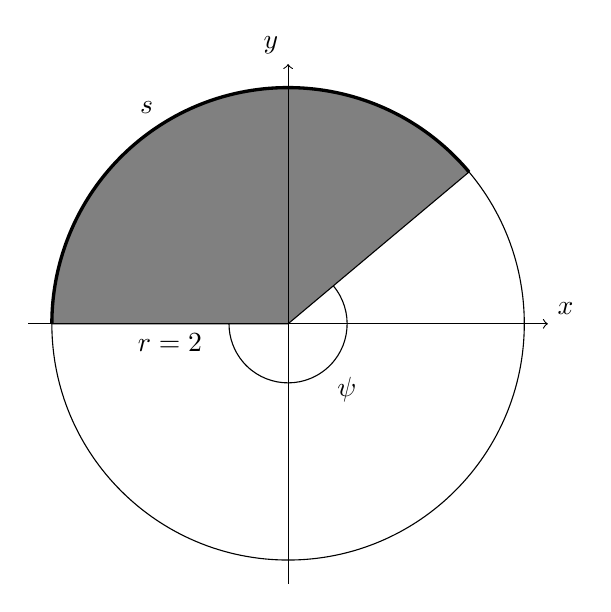
\begin{tikzpicture}[y=1.5cm, x=1.5cm,font=\sffamily]
    \draw[thin,black,fill=gray] (0,0) -- (40:2) arc (40:180:2) -- (0,0);
    \draw[very thick,black] (40:2) arc (40:180:2);
    \draw[black] (0,0) circle (2);
    \draw[black] (40:0.5) arc (40:-180:.5) node[pos=0.4,anchor=north west] {$\psi$};
    \draw[thin,black,->] (-2.2,0.0) -- (2.2,0.0) node[anchor=south west] {$x$};
    \draw[thin,black,->] (0.0,-2.2) -- (0.0,2.2) node[anchor=south east] {$y$};
    \node[black,anchor=north] at (-1,0) {$r=2$};
    \node[black,anchor=south east] at (122:2) {$s$};
  \end{tikzpicture}


\item A race track is in the shape of a circle, and the inside
  diameter of the track is 0.8km. A cart goes around the track eight
  and a half times hugging the inside of the track, and the diameter
  of its rear wheel is 0.3m. (1000m=1km) What angle did the rear wheel
  turn? If the diameter of the track is increased what will happen to
  the angle?

\item A researcher performed an experiment with three
  species of mole. For each subject she measured its mass and cardiac
  output. A polar plot will be constructed. The angles are based on
  the average masses of the three species, and the areas of each
  sector are based on the average cardiac output of the three
  species. She determines that the angle for the first species,
  $\theta$, should be 15\% of the circle, and the angle for the second
  species, $\alpha$, should be 40\% of the circle. She also determines
  that the area of the sector for the first species should be 1
  m\textsuperscript{2}, the area of the sector for the second species
  should be 2 m\textsuperscript{2}, and the area of the sector for the
  third species should be 3 m\textsuperscript{2}. Determine the
  values of the three angles and the three radii.

  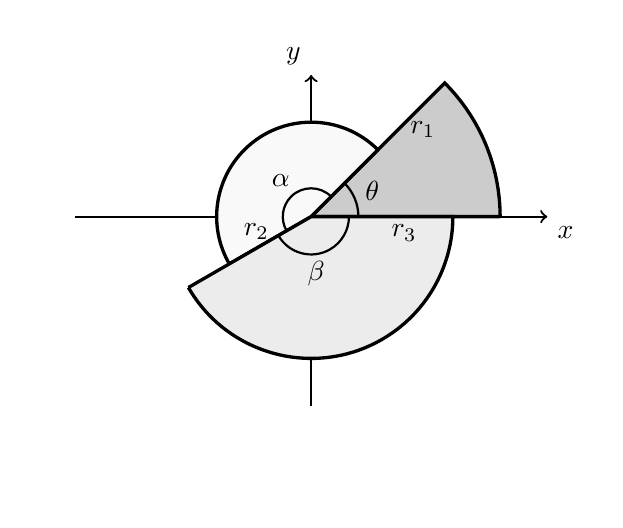
\begin{tikzpicture}[y=1.2cm, x=1.2cm,font=\sffamily]
    % Define the x  bounds
    \def\lowX{-2.5}
    \def\highX{2.5}
    % Define the  y bounds
    \def\lowY{-2.0}
    \def\highY{1.5}

    %\draw[step = 1, gray, very thin,opacity=0.5] (\lowX, \lowY) grid ( \highX, \highY);
        % axis
        \draw[thick,->] (\lowX,0) -- coordinate (x axis mid) (\highX,0) node[anchor = north west] {$x$};
    \draw[thick,->] (0,\lowY) -- coordinate (y axis mid) (0,\highY) node[anchor = south east] {$y$};

    % Add a plot of the path.
    \begin{scope}
      \clip(-3,-3) rectangle ++(6,5);
      \draw[scale=1.0,smooth,very thick,black,fill=gray!40]  (0:2) arc (0:45:2) -- (0,0) -- (0:2);
      \draw[scale=1.0,smooth,thick,black]  (0:0.5) arc (0:45:0.5);
      \draw[scale=1.0,smooth,very thick,black,fill=gray!5]  (45:1) arc (45:210:1) -- (0,0) -- (45:1);
      \draw[scale=1.0,smooth,thick,black]  (45:0.3) arc (45:210:0.3);
      \draw[scale=1.0,smooth,very thick,black,fill=gray!15]  (210:1.5) arc (210:360:1.5) -- (0,0) -- (210:1.5);
      \draw[scale=1.0,smooth,thick,black]  (210:0.4) arc (210:360:0.4);
    \end{scope}

   % Add the annotations to the plot.
    \node at (22.5:0.7) {$\theta$};
    \node at (130:0.5) {$\alpha$};
    \node at (275:0.6) {$\beta$};
    \node at (38:1.5) {$r_1$};
    \node at (195:0.6) {$r_2$};
    \node at (350:1.0) {$r_3$};

  \end{tikzpicture}



\end{enumerate}


\preClass{Coordinate Systems}


\videoLink{Section 4.2 day 1}{https://www.youtube.com/playlist?list=PLYHZK3b8UFw2_C72_BEthTH-k3sKuNAEb}

\begin{enumerate}
\item  Suppose that the real number $t$ corresponds to the point $\displaystyle P\Big(-\frac{\sqrt{13}}{4},\frac{\sqrt{3}}{4}\Big)$ on the unit circle.  Evaluate the six trigonometric functions at $t$.
\begin{enumerate}

\item $\sin(t)=$\vfill
\item $\cos(t)=$\vfill
\item $\tan(t)=$\vfill
\item $\csc(t)=$\vfill
\item $\sec(t)=$\vfill
\item $\cot(t)=$\vfill
\end{enumerate}




\newpage


\item Use the coordinates on the unit circle to find the value of each trig function at the indicated real number.
\begin{enumerate}
\item $\displaystyle \sin\Big(\frac{4\pi}{3}\Big)=$\vfill
\item $\displaystyle \csc\Big(\frac{4\pi}{3}\Big)=$\vfill
\end{enumerate}

\item  Evaluate the trig functions at the indicated real number.
\begin{enumerate}
\item $\displaystyle \cos\Big(-\frac{\pi}{6}\Big)=$\vfill
\item $\displaystyle \tan\Big(-\frac{\pi}{6}\Big)=$\vfill
\end{enumerate}




\end{enumerate}




\include{angles/Worksheet-4.2a}

\preClass{Coordinate Systems}



\noindent Watch the Pre-Class videos for Section 4.2B and answer the following questions. Remember that in your written work you are graded on the correctness of your supporting work and not just your final answer. Always give an exact answer unless you are explicitly told to round; calculator approximations will not receive full credit. 


\begin{enumerate}
\item  Evaluate the functions if possible.  Your answers must be exact and not decimal approximations.

\begin{enumerate}

\item $\sin(0)=$\vfill
\item $\cot(\pi)=$\vfill
\item $\tan(3\pi)=$\vfill
\item $\sec(\pi)=$\vfill
\item $\csc(0)=$\vfill
\item $\cos(\pi)=$\vfill
\end{enumerate}




\newpage


\item  Given $ \displaystyle \cos(t)=\frac{7}{25}$ for $\displaystyle \frac{3\pi}{2}<t<2\pi$.  Use an appropriate Pythagorean Identity to find the value of $\sin(t)$.\vfill

\item  Circle all properties that apply to $\csc(t)$.
\begin{enumerate}
\item The function is even.
\item The function is odd.
\item The period is $2\pi$.
\item The period is $\pi$.
\item The domain is all real numbers.
\item The domain is all real numbers excluding odd multiples of $\frac{\pi}{2}$.
\item The domain is all real numbers excluding multiples of $\pi$.
\end{enumerate}



\end{enumerate}




\include{angles/Worksheet-4.2b}

%%% Local Variables:
%%% mode: latex
%%% TeX-master: "../labManual"
%%% End:
